\documentclass[]{report}
\usepackage{kotex}
\usepackage{verbatim} 
\usepackage{graphicx} 

\usepackage{listings}
\usepackage{color}

\definecolor{dkgreen}{rgb}{0,0.6,0}
\definecolor{gray}{rgb}{0.5,0.5,0.5}
\definecolor{mauve}{rgb}{0.58,0,0.82}

\lstset{frame=tb,
	language=Python,
	aboveskip=3mm,
	belowskip=3mm,
	showstringspaces=false,
	columns=flexible,
	basicstyle={\small\ttfamily},
	numbers=none,
	numberstyle=\tiny\color{gray},
	keywordstyle=\color{blue},
	commentstyle=\color{dkgreen},
	stringstyle=\color{mauve},
	breaklines=true,
	breakatwhitespace=true,
	tabsize=3
}


% Title Page
\title{HW06 - REPORT}
\author{정보컴퓨터공학부 201624536 이국현}


\begin{document}
\maketitle


\chapter{서론}
\begin{itemize}
	\item Fundamental matrix
	\item Epipole
	\item Epipolar line
\end{itemize}

\section{Fundamental matrix}

\[ x'^TFx = 0 \]

Fundamental matrix는 위 식을 만족하는 F이다. 여기서 $ x=(u,v,1)^T $를 $ x'=(u',v',1)^T $라고 하면 다음과 같이 나타낼 수 있다. \\

\begin{figure}[ht!]
    \centering
    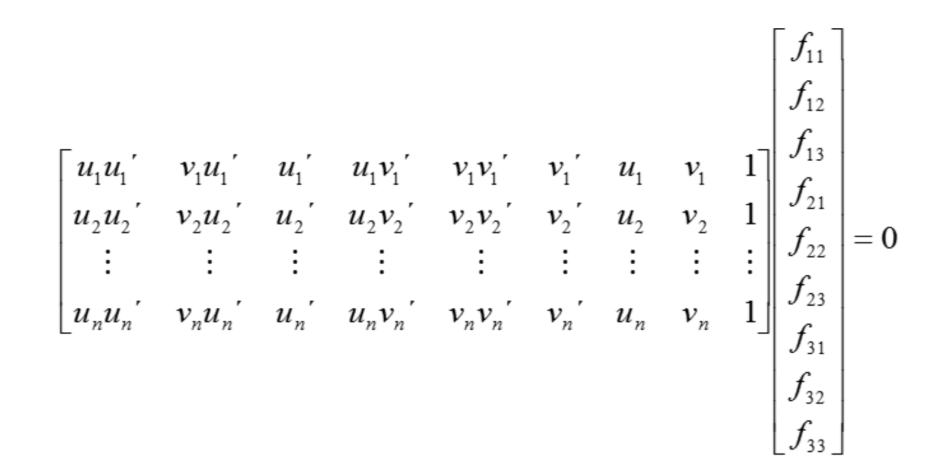
\includegraphics[width=0.9\textwidth]{image/matrix.png}
    \caption{Fundamental matrix}
    \label{matrix}
\end{figure}



\section{Epipole}

Epipole은 Epipolar line 위에 있기 때문에 다음과 같은 식을 만족한다. \\

\[ Fe_1 = 0 \]
\[ Fe_2 = 0 \]

\section{Epipolar line}

\begin{figure}[ht!]
    \centering
    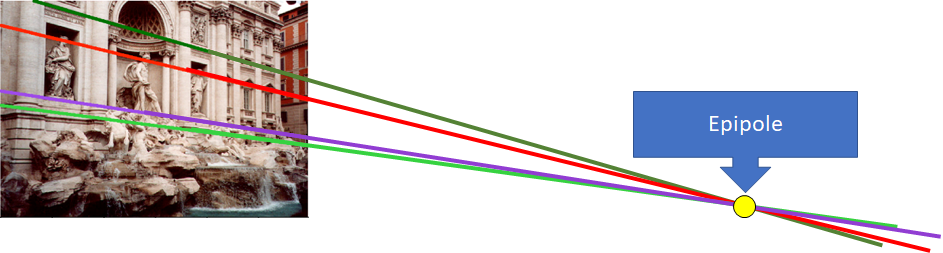
\includegraphics[width=0.9\textwidth]{image/epipolar_line.png}
    \caption{Epipolar line}
    \label{epipolarline}
\end{figure}

Epipole과 feature를 연결하면 Epipolar line을 생성할 수 있다. \\


\chapter{본론}

\section{compute\_fundamental}


\begin{lstlisting}
def compute_fundamental(x1, x2):
	n = x1.shape[1]
	if x2.shape[1] != n:
		exit(1)
	
	F = None
	# YOUR CODE BEGINS HERE
	
	# build matrix for equations in Page 51
	A = np.empty((0, 9))
	for k in range(n):
		row = np.outer(x1.T[k], x2.T[k]).flatten()
		A = np.append(A, [row], axis=0)
	# compute the solution in Page 51
	
	# SVD를 사용하여 최소화 eigenvector를 구함
	F = np.linalg.svd(A)[2][-1]
	F = F.reshape((3, 3))
	
	# constrain F: make rank 2 by zeroing out last singular value (Page 52)
	# SVD를 사용하여 분리
	U, sigma, V_t = np.linalg.svd(F)
	sigma = np.diag(sigma)
	sigma[2][2] = 0 # homogeneous to 2d
	F = U @ sigma @ V_t  # F = U.dot(sigma).dot(V_t)
	
	# YOUR CODE ENDS HERE
	
	return F
\end{lstlisting}

Fundamental matrix를 구하기 위해 x1, x2를 이용하여 A matrix를 구현하였다. 
그리고 $AF=0$를 만족하는 F를 찾기 위해 SVD를 사용하여 $||AF||$를 최소화하는 Fundamental matrix F를 찾았다. 
마지막으로 Homogeneous의 Fundamental matrix를 2D로 변환하기 위해 SVD를 통해 분리하고, 3D 요소를 없애준 뒤 다시 결합하였다. \\



\section{compute\_epipoles}

\begin{lstlisting}
def compute_epipoles(F):
	e1 = None
	e2 = None
	# YOUR CODE BEGINS HERE
	# SVD를 사용하여 최소화 eigenvector를 구함
	e1 = np.linalg.svd(F)[2][-1]
	e2 = np.linalg.svd(F.T)[2][-1]
	e1 = e1 / e1[-1]
	e2 = e2 / e2[-1]
	# YOUR CODE ENDS HERE
	
	return e1, e2
\end{lstlisting}

SVD를 이용하여 각 이미지의 $ Fe_1 = 0 $에서 Epipole e를 계산한다.  \\


\section{draw\_epipolar\_lines}

\begin{lstlisting}
	def draw_epipolar_lines(img1, img2, cor1, cor2):
    F = compute_norm_fundamental(cor1, cor2)

    e1, e2 = compute_epipoles(F)
    # YOUR CODE BEGINS HERE
    plt.subplot(1, 2, 1)
    plt.imshow(img1)
    # 그릴 epipolar line의 x domain
    X = np.linspace(0, img1.shape[0], img1.shape[0] + 1)
    for i, p1 in enumerate(cor1.T):
        color = colors[i % len(colors)]  # line 마다 다른 색상 사용
        # epipolar line을 그리기 위한 기울기
        gradient = (e1[1] - p1[1]) / (e1[0] - p1[0])
        # epipolar line을 y절편
        intercept = e1[1] - gradient * e1[0]
        # 그릴 epipolar line의 y domain
        Y = gradient * X + intercept
        plt.scatter(p1[0], p1[1], color=color)
        plt.plot(X, Y, color=color)
    # ------------------------------------------------------
    plt.subplot(1, 2, 2)
    plt.imshow(img2)
    # 그릴 epipolar line의 x domain
    X = np.linspace(0, img2.shape[0], img2.shape[0] + 1)
    for i, p2 in enumerate(cor2.T):
        color = colors[i % len(colors)]
        # epipolar line을 그리기 위한 기울기
        gradient = (e2[1] - p2[1]) / (e2[0] - p2[0])
        # epipolar line을 y절편
        intercept = e2[1] - gradient * e2[0]
        # 그릴 epipolar line의 y domain
        Y = gradient * X + intercept
        plt.scatter(p2[0], p2[1], color=color)
        plt.plot(X, Y, color=color)
    plt.show()
    # YOUR CODE ENDS HERE

    return
\end{lstlisting}

이미지의 Feature와 Epipole을 연결하여 Epipolar line을 그려 주었다. 
두 점을 가지고 기울기와 y 절편을 구하고 matplotlib을 통해 plot line을 구려주었다. \\

\chapter{결론}

\begin{figure}[ht!]
    \centering
    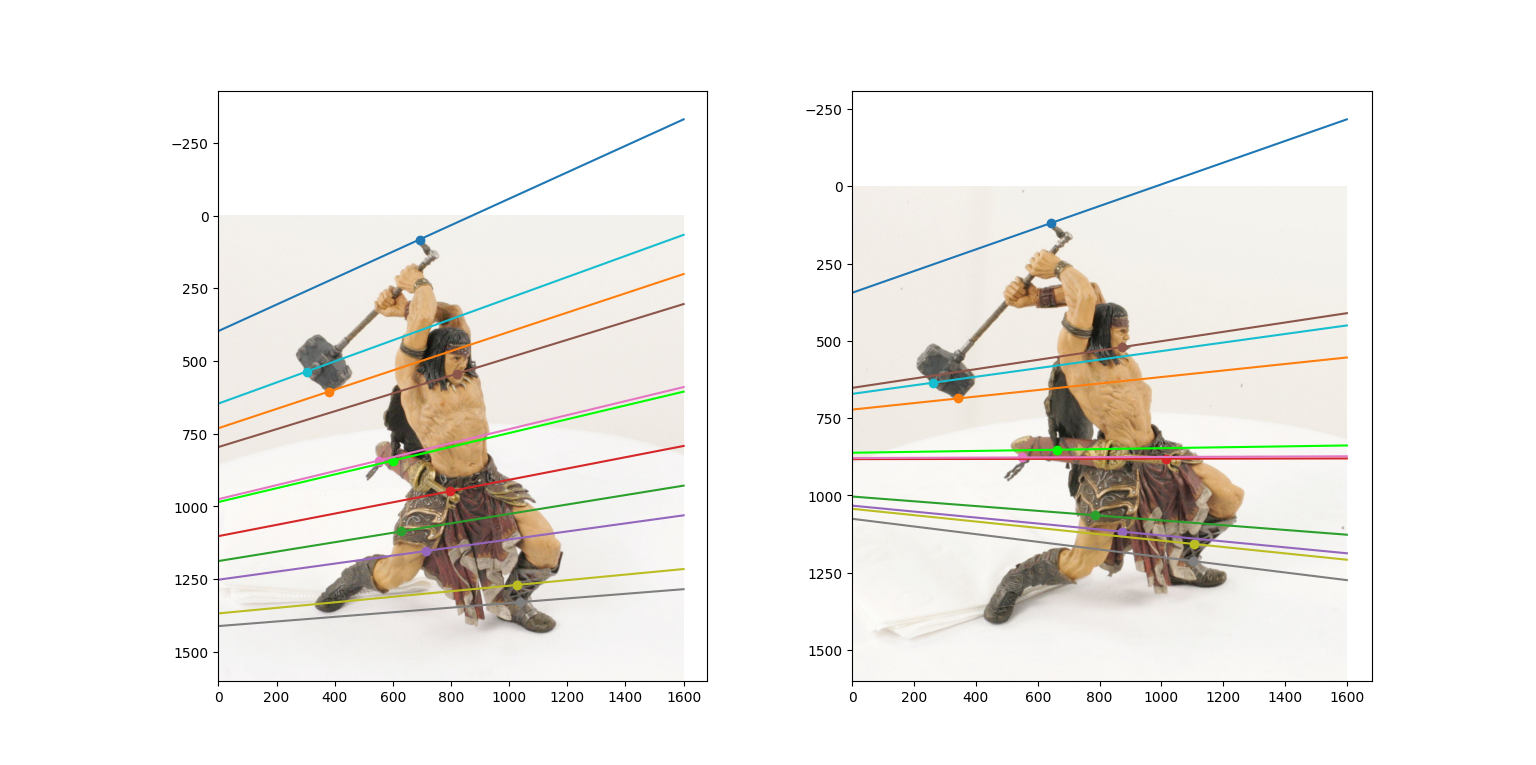
\includegraphics[width=1.0\textwidth]{image/result.png}
    \caption{Epipolar line}
    \label{Epipolar}
\end{figure}

Feature들을 통해 Fundamental matrix를 구하고 이 Fundamental matrix를 통해 Epiple을 구하였다. 
구한 Epipole과 Feature를 연결하여 Epipolar line을 그려 보니 모든 Feature의 Epipolar line이 가상의 한 점에서 모이는 것을 확인할 수 있다.  \\

\end{document}          
